\documentclass[12pt]{article}
\textwidth 16.5cm \oddsidemargin 0cm \topmargin -2.3cm \textheight
25.3cm \footskip 1.5cm
\usepackage{spverbatim,graphicx}
\begin{document}
\section*{Appendix A: Example definition files}


\begin{picture}(0,0)
	\put(120,-190){\hbox{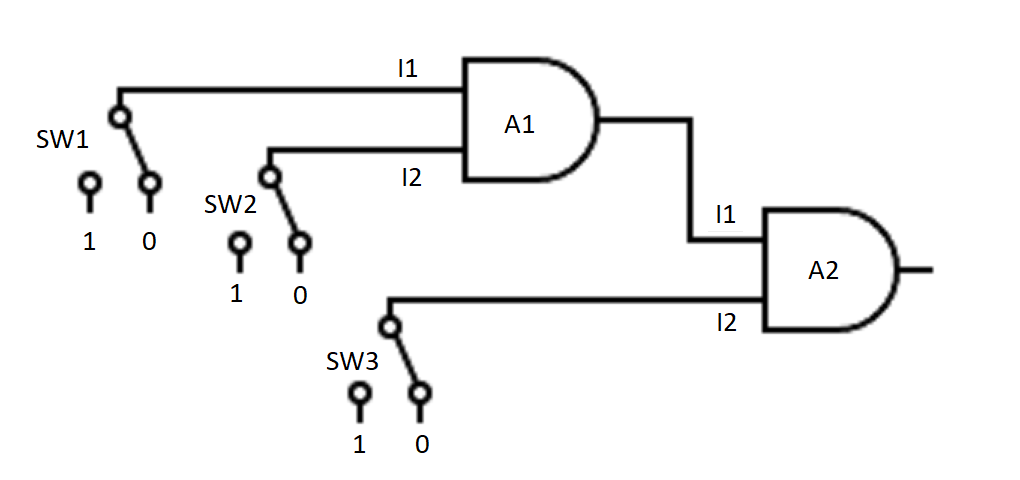
\includegraphics[scale=0.8]{first_example}}}
\end{picture}
\subsection*{First example definition file}
\begin{spverbatim}
	DEVICES:
	SWITCH SW1 0,
	SWITCH SW2 0,
	SWITCH SW3 0,
	AND A1 2,
	AND A2 2;
	CONNECTIONS:
	SW1->A1.I1,
	SW2->A1.I2,
	SW3->A2.I2,
	A1->A2.I1;
	MONITOR:
	A1, A2;
\end{spverbatim}


\begin{picture}(0,0)
	\put(110,-250){\hbox{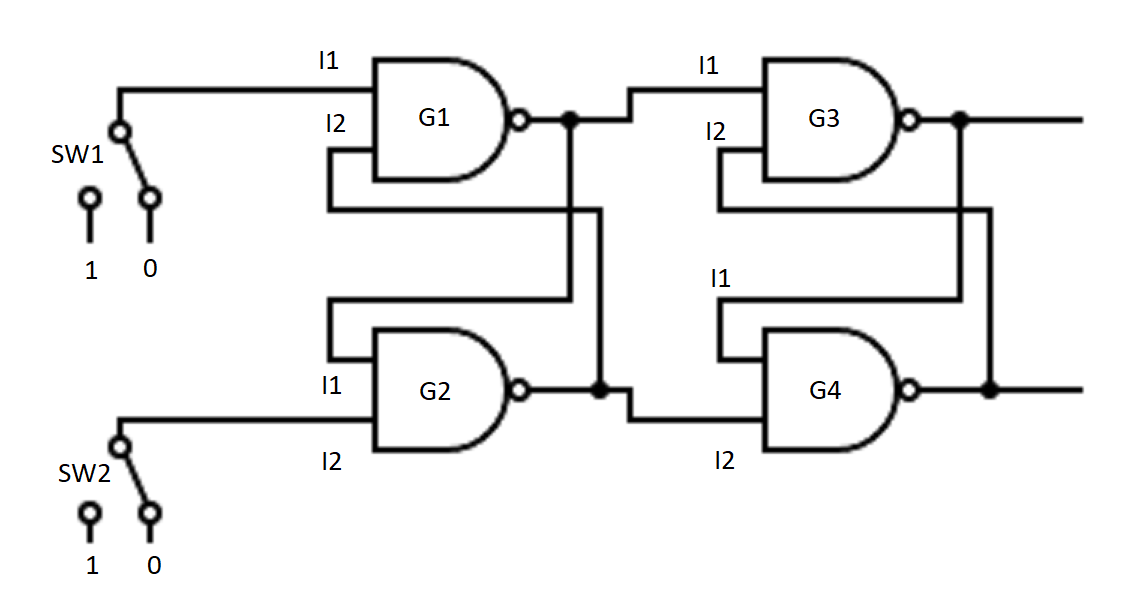
\includegraphics[scale=0.8]{second_example}}}
\end{picture}
\subsection*{Second example definition file}
\begin{spverbatim}
	DEVICES:
	SWITCH SW1 0,
	SWITCH SW2 0,
	NAND G1 2,
	NAND G2 2,
	NAND G3 2,
	NAND G4 2;
	CONNECTIONS:
	SW1->G1.I1,
	SW2->G2.I2,
	G1->G2.I1,
	G2->G1.I2,
	G1->G3.I1,
	G2->G4.I2,
	G3->G4.I1,
	G4->G3.I2;
	MONITOR:
	G1, G2, G3, G4;
\end{spverbatim}

\newpage
\begin{picture}(0,0)
	\put(110,-400){\hbox{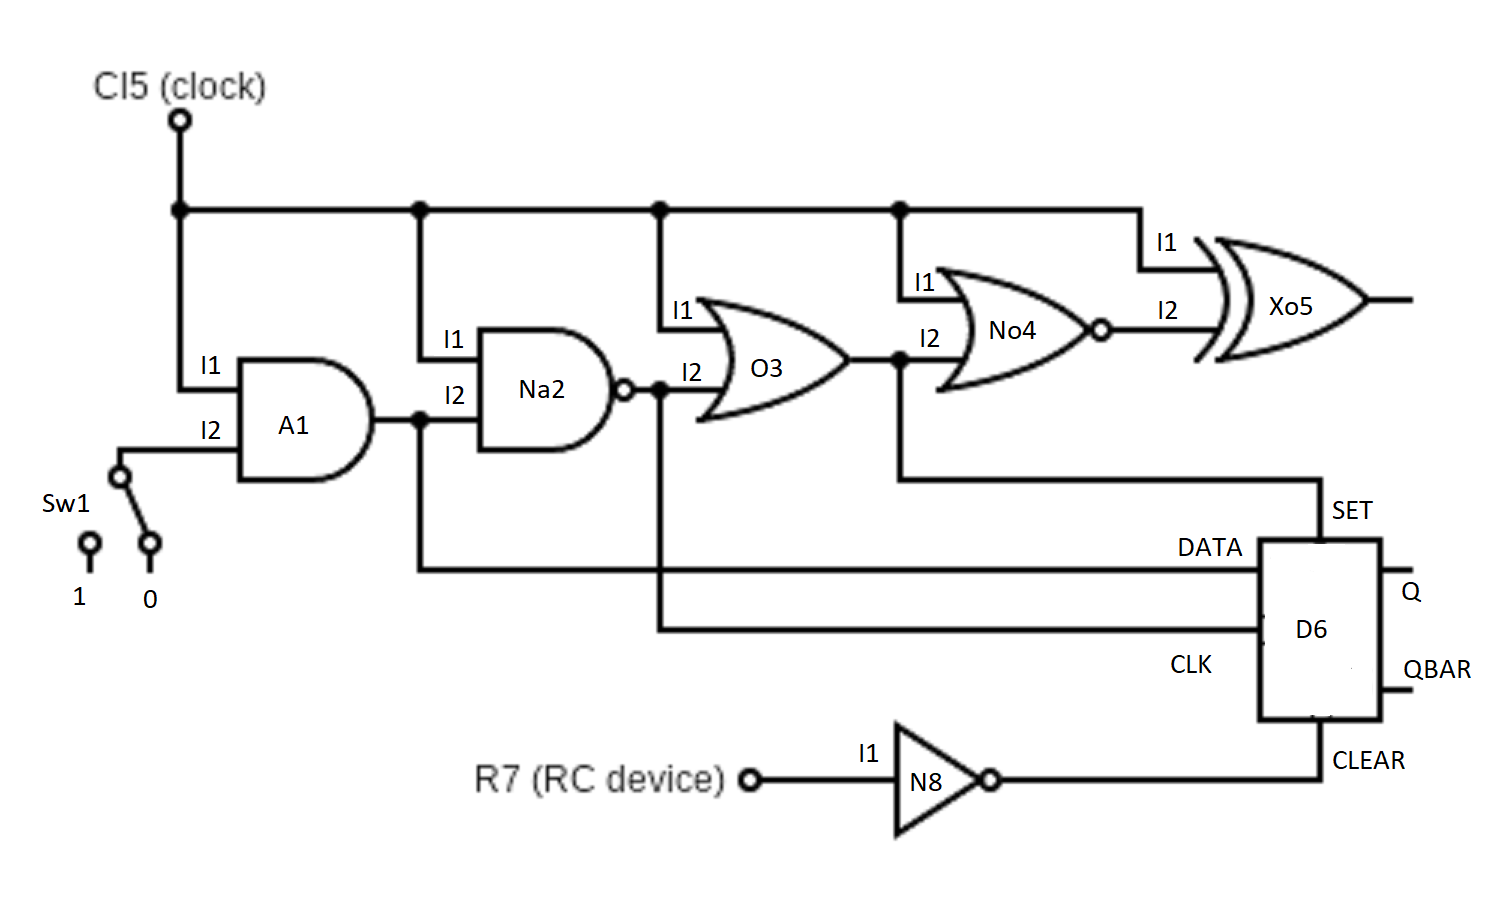
\includegraphics[scale=0.7]{circuit}}}
\end{picture}
\subsection*{Third example definition file}
\begin{spverbatim}
	\\ Fit in all the supported DEVICES
	DEVICES: \* Each device in DEVICES is one of the following:
	SWITCH, CLOCK, AND, NAND, OR, NOR, XOR, DTYPE.
	DEVICES list is the first one to be parsed. *\
	\\ ->Basics<-
	CLOCK Cl5 5,
	SWITCH Sw1 0,
	\\?Gates?
	AND A1 2,
	NAND Na2 2,
	OR O3 2,
	NOR No4 2,
	\\*No parameter ones*
	XOR Xo5,
	DTYPE D6,
	\\ *\ New devices
	RC R7 3,
	NOT N8;

	CONNECTIONS:
	Cl5 -> A1.I1,
	Cl5 -> Na2.I1,
	Cl5 -> O3.I1,
	Cl5 -> No4.I1,
	Cl5->Xo5.I1,
	Sw1 -> A1.I2,
	A1 -> Na2.I2,
	Na2   ->    O3.I2,
	O3 -> No4.I2,
	No4 -> Xo5.I2,
	A1 -> D6.DATA,
	Na2 -> D6.CLK,
	O3 -> D6.SET,
	R7 -> N8.I1,
	N8 -> D6.CLEAR;

	MONITOR:
	A1, Na2, O3, No4, Xo5, D6.Q, D6.QBAR, R7, N8;
\end{spverbatim}

\end{document}
